\chapter{Device fabrication}

\section{General overview}


The aim of our fabrication step is to obtain a structure suitable for a single molecule transistor geometry. This typical geometry is depicted on figure \ref{fig:SMT_picture}. The main challenges in that kind of geometry can be summarized as follow :

\begin{list}
  \item obtain a good coupling of the gate 
  \item produce a small gap of the size of the molecule
\end{list}

\begin{figure}[h]
  \begin{center}
    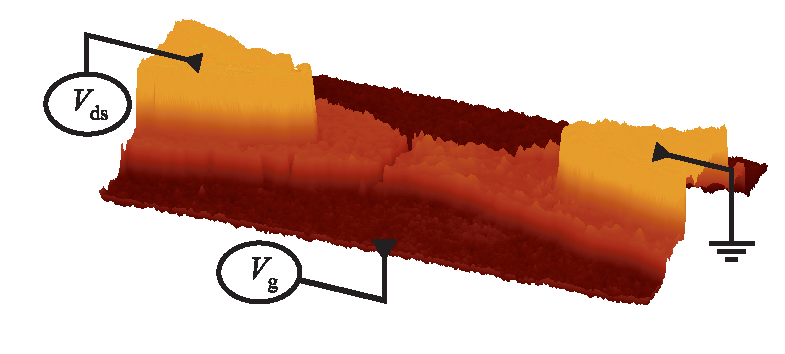
\includegraphics[width = 12cm]{fabrication_chapter/figs/SMT.eps}
  \end{center}
  \caption{3D extrapolation of a 2D Scanning Tunneling Microscope (SEM) image.}
  \label{fig:SMT_picture}
\end{figure}

\section{Lithographic steps}
\section{Electromigration technique}
\section{Toward high-k oxides: the ALD technique}

